\chapter{Robô}
\label{ch:identificador}

\section{Apresentação Steve Robot Express}

Nós da Drop Flash realizamos além das entregas já mencionadas o serviço de entregas voltada para condomínios comerciais, residências e Shoppings centers chamado Steve Robot Express. Com a Steve Robot Express disponibilizamos aluguéis de robôs de quatro rodas que se movem livremente realizando a entregas    de comida documentos e pequenos pacotes até trinta quilos atendendo as necessidades dos nossos clientes. Usado em um condomínio por exemplo o robô Steve poderia realizar a emprega de pedidos sem a necessidade de o morador descer até a portaria pois o Steve faria isso para você trazendo o pedido até sua porta trazendo mais conforto e praticidade otimizando o tempo de todos, o morador teria apenas que solicitar o serviço por meio de um aplicativo de smartphone e utilizar o mesmo para desbloquear e abrir o compartimento de carga e retirar o seu pedido \cite{BoysenN2018}.

Para implantação do Steve em um condomínio levaremos em conta a quantidade de residências, pedidos recebidos em um mês, distância percorrida e tempo máximo de entrega para a unidade mais longe. Com esses dados conseguimos mensurar a quantidade de robôs a serem instalados.

Em uma implantação que realizamos em um condomínio de 328 unidades com 1.387 pedidos recebidos na portaria por mês chegamos na média de 4,2 pedidos por unidade, calculando que o tempo máximo de entrega para a moradia mais longe seria de 10 minutos, com todos esses dados realizamos o cálculo do tempo mensal de entregas = 328 x 4,2 x 10 chegamos no resultado de 13.776 minutos. Nosso robô Steve tem autonomia de 12 horas mas para garantir uma maior durabilidade eles trabalham apenas 8 horas por dia o que seria equivalente a 480 minutos por dia ou 14.400 minutos por mês sabendo disso realizamos o ultimo cálculo para saber quantos robôs são necessários para atender o condômino 13.776 / 14.400 chegamos ao resultado de 0,95 a arredondando chegamos à conclusão de que seira necessário um robô para realizar as entregas em todas as 328 unidades do condomínio mas por motivos de segurança e picos de pedidos recebidos em horas especificas orientamos a instalação de duas unidades do Steve para uma entrega mais rápida e dinâmica.

O Steve também conta com diversas funcionalidades projetado para otimizar o processo de entregas funciona de forma autônoma com uma tecnologia que conta com mais de dez câmeras garantindo uma visão de trezentos e sessenta graus, sensores ultrassônicos, navegação GPS, permitindo que a inteligência artificial detecte obstáculos e tome decisões, como desviar ou parar até que um obstáculo móvel passe. Nosso Robô Steve também consegue diferenciar calçadas, ruas, grama, ciclovia e árvores, mesmo em ambientes externos. Steve também conta com sistemas de comunicação (IoT) Internet das coisas e (M2M) Machine-to-Machine sendo o M2M fundamental na IoT, permitindo que dispositivos troquem informações diretamente entre si, sem intervenção humana montando uma memória colaborativa de rotas, com o objetivo de criar uma navegação autônoma cada vez mais precisa criando um mapa com características especificas dos ambientes tornando as viagens cada vez mais rápidas, Além de garantir uma interação maior com outros equipamentos eletrônicos no caso do Steve seria a comunicação com sistemas de elevadores permitindo sua movimentação sem problemas em todos os andares do edifício. Garantindo assim total autonomia do Steve a implantação do sistema IoT nos elevadores e feita em conjunto com a Dusun IoT \cite{DusunIot} especializada em hardware e gateways IoT fornecendo todos os dispositivos necessários. Já os pontos de recarga são instalados em conjunto com a Synkar, companhia brasileira especializada em inteligência artificial que disponibiliza toda a parte de software, automação, manutenção e reposição de peças sendo ela a responsável por fabricar e disponibilizar todos os robôs Steve. Visando também na diminuição dos impactos ambientais todos os robôs produzidos são 100\% elétricos os tornando ecologicamente corretos, contribuindo para a redução das emissões de gases do efeito estufa (GEE) e também do congestionamento em grandes cidades \cite{Bakach2020}

\section{Especificações do Steve} 
\begin{figure} [!ht]
   { \centering
    \caption{Ilustração robô de entregas da empresa Synkar}
    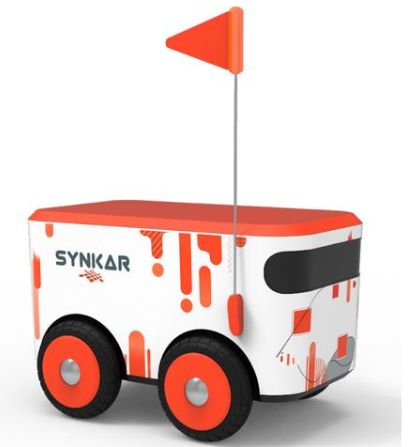
\includegraphics[width=0.5\linewidth]{figuras/synkar.png}
    \label{fig:enter-label}
    \fonte{https://www.synkar.com/ourrobots/}
    }
\end{figure}

Capacidade de transporte: 30 kg Veículo: 100\% elétrico
Autonomia: 12 horas Navegação: Autônoma por Inteligência Artificial
Sistema: Machine-to-Machine Atuação na primeira e Última milha
API: Drop Flash Steve API (DFSA) Fabricante: Synkar

\section{Logística Interna e Externa}
Compreendemos que as operações do mundo real não se restringem a um único cenário. Portanto, nossos robôs têm a capacidade de operar tanto em ambientes internos quanto externos.

\begin{figure} [!ht]
    {\centering
    \caption{Diferentes formas de interpretação dos ambientes através de câmeras}
    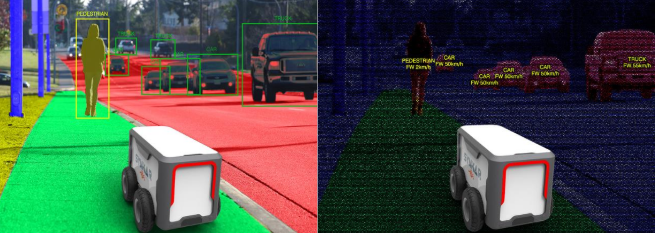
\includegraphics[width=0.5\linewidth]{figuras/stevelogistica.png}
    \label{fig:enter-label}
    \fonte{https://www.synkar.com/ourrobots/}
    }
\end{figure}

\section{Navegação Por Inteligência artificial}
Acreditamos que a automação está moldando o futuro. Nossos robôs têm a capacidade de proporcionar segurança, rapidez e consistência nas operações dos nossos parceiros.

\begin{figure}[!ht]
   { \centering
    \caption{Demonstração da capacidade de tomada de decisão ao encontrar obstáculos}
    \includegraphics[width=0.5\linewidth]{figuras/stevenavegaçao.png}
    \label{fig:enter-label}
    \fonte{https://www.synkar.com/ourrobots/}
    }
\end{figure}

\section{API customizável para os parceiros}
A Drop Flash Steve API (DFSA) é altamente flexível e pode ser adaptada às necessidades específicas dos nossos parceiros. Ela oferece desde operações logísticas básicas até a possibilidade de desenvolver funcionalidades personalizadas.

\section{Curiosidades}
Escolhemos o nome de Steve para o nosso robô em homenagem a Steve Jobs que com seus feitos revolucionou a área da tecnologia deixando seu legado e servindo de exemplo para as novas gerações por sua criatividade e visão que moldaram a forma com interagimos com a
tecnologia até hoje. Nós da Drop Flash seguimos o mesmo caminho revolucionando na área de entregas buscando a cada dia trazer mais economia de tempo e praticidade aos nossos clientes com novas tecnologias sustentáveis.